\subsection{Effect of number of training data points on map output} \label{subsec:num_train}

To understand how the number of training data points affect the map output, another map (Map 7) was created with the same range of training data as Map 1 and 24 data points only, as shown in Figure~\ref{fig:map_1_7_training_data}. The accuracy of Map 7 is compared with that of Map 1 in Table \ref{tb:map7_acc}.

\begin{table}[h]
\caption{\label{tb:map7_acc}Coefficients of variation of Maps 1 and 7.}
\begin{center}
\begin{tabular}{p{1.2cm} p{6cm} p{5.3cm}}
\br
Map & Coefficient of variation based on training data poinst only ($cov_{train}$) & Coefficient of variation based on all available data points ($cov_{all}$) \\
\mr
Map 1&0.18\%&0.31\%\\
Map 7&0.17\%&1.15\%\\
\br
\end{tabular}
\end{center}
\end{table}

Table \ref{tb:map7_acc} shows that the accuracy of Map 7 is similar to that of Map 1 at the training data points, but the analysis with all available data points shows that Map 7 is less accurate than that of Map 1. This shows that despite similar range of training data, fewer training data points reduces map accuracy. But to know if the reduction of accuracy happens at extrapolation, the accuracy of the map outputs is compared with the uncertainty from model random error and the uncertainty from training data as shown in Figures \ref{fig:num_train_model} and \ref{fig:num_train_train}.

\begin{figure}[h]
\begin{minipage}{15pc}
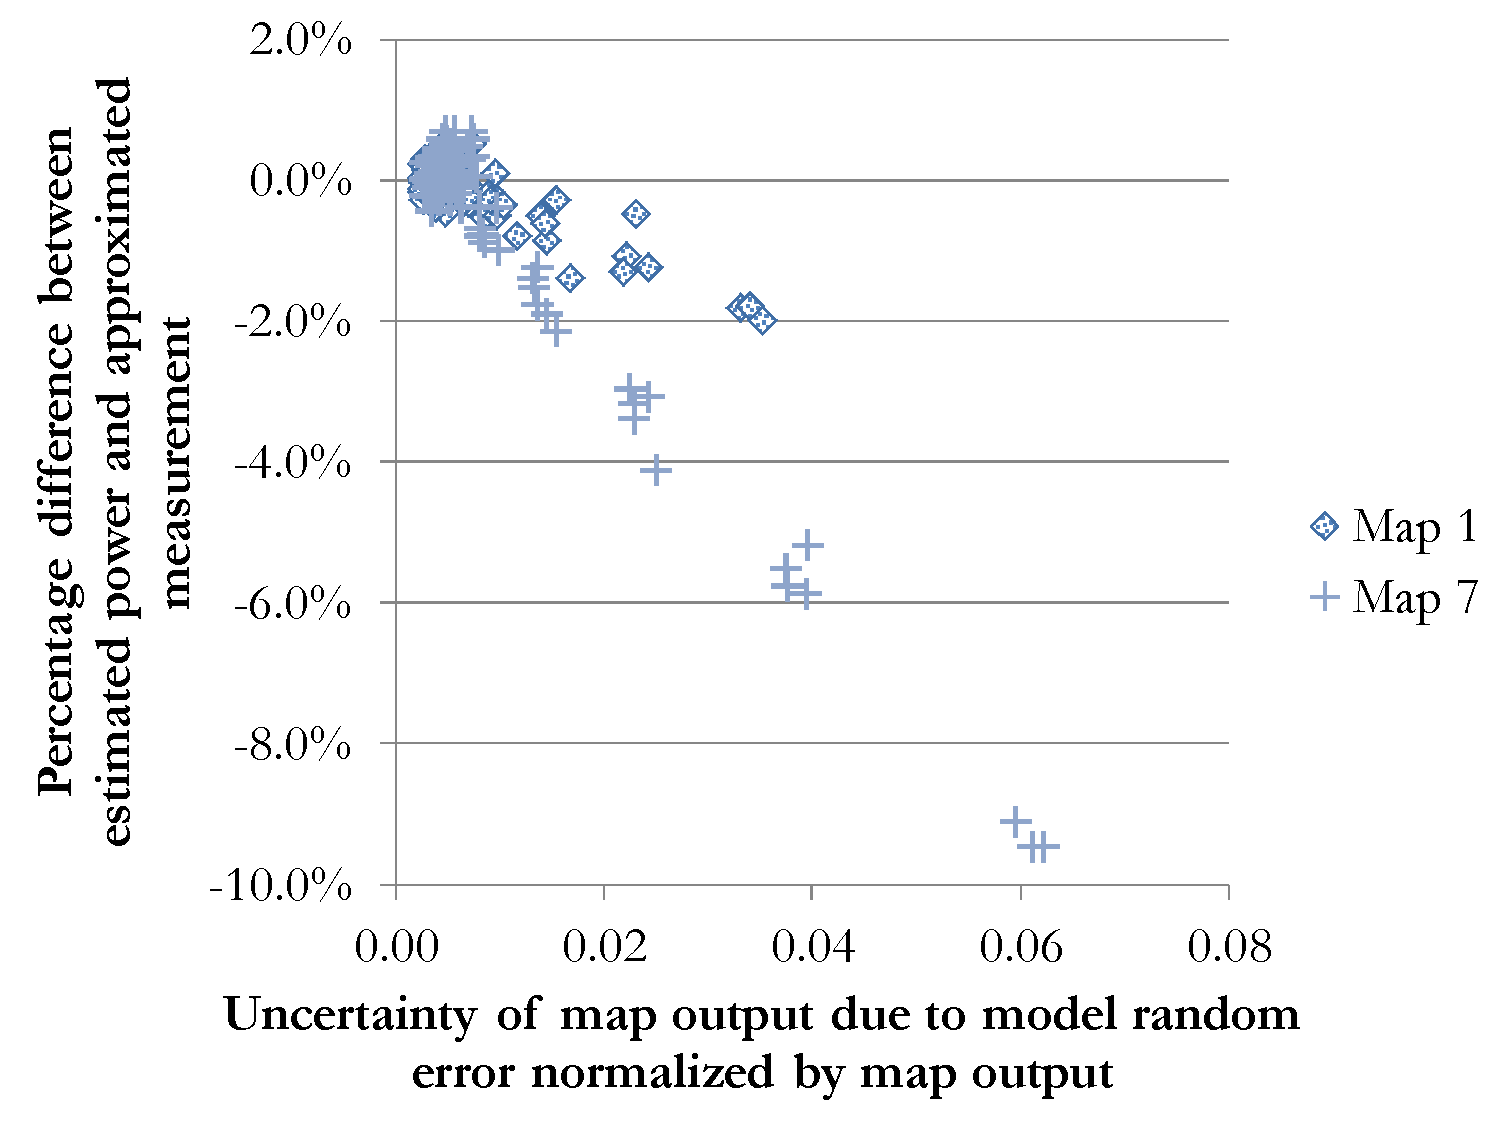
\includegraphics[width=15pc]{num_train_model.pdf}
\caption{\label{fig:num_train_model}Change of accuracy of maps with uncertainty from model random error in Maps 1 and 7.}
\end{minipage}\hspace{2pc}%
\begin{minipage}{15pc}
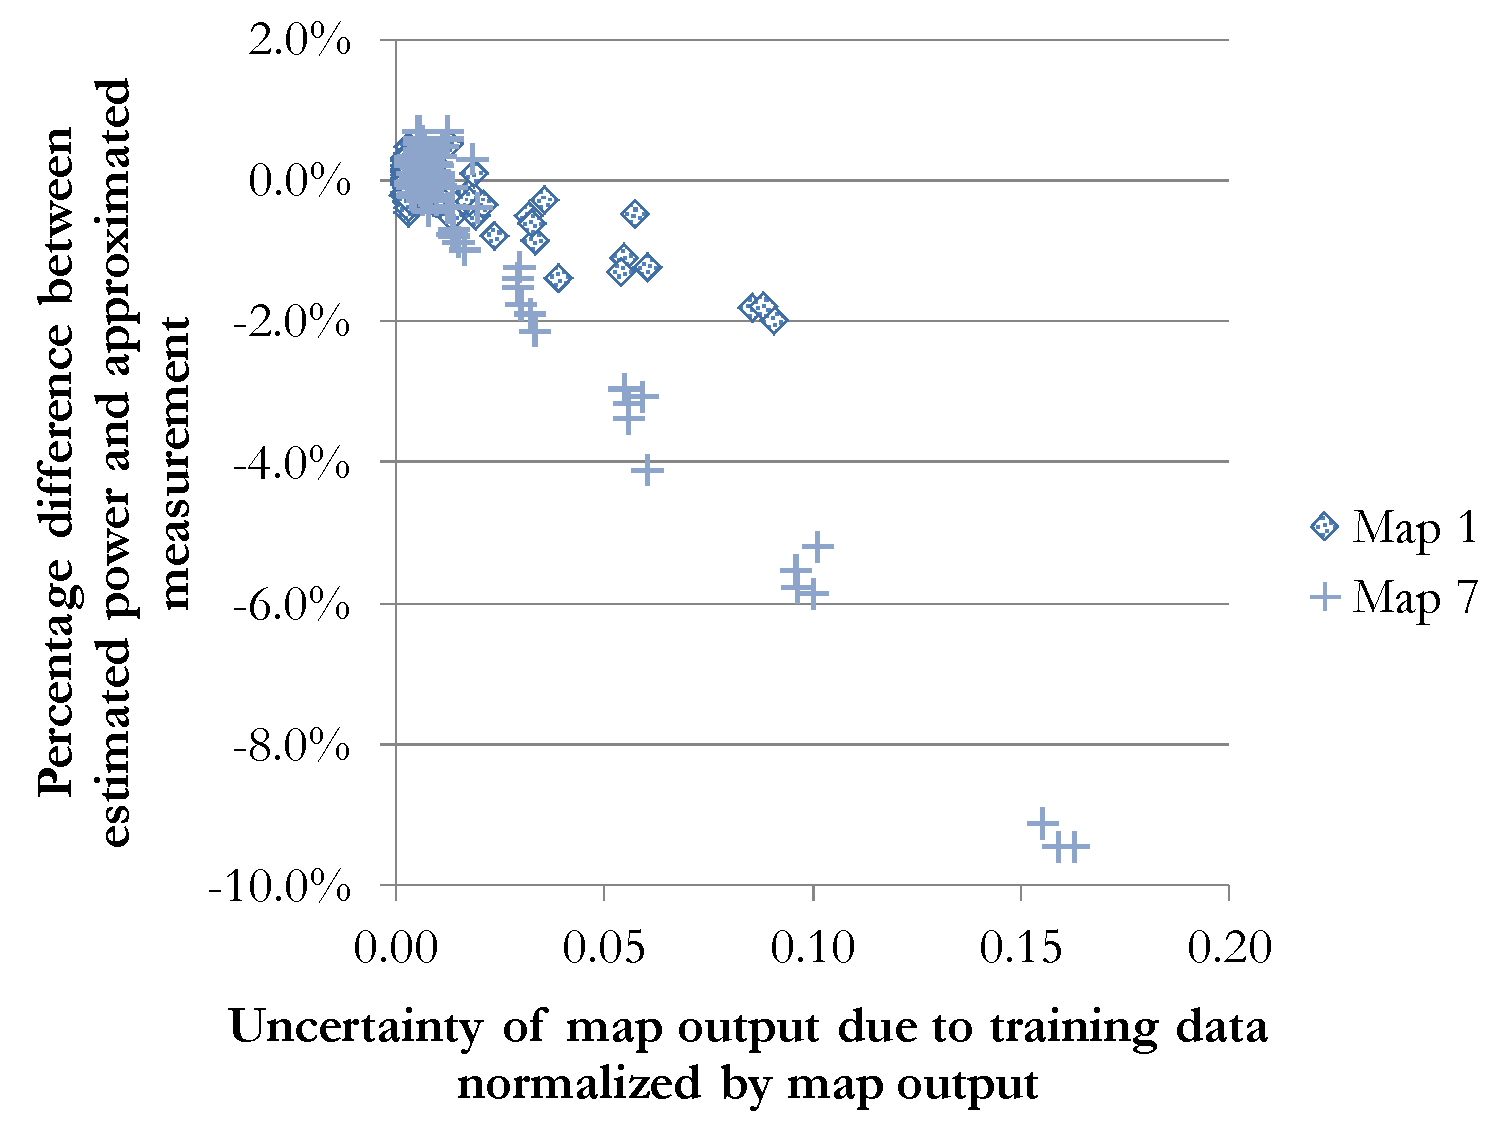
\includegraphics[width=15pc]{num_train_train.pdf}
\caption{\label{fig:num_train_train}Change of accuracy of maps with uncertainty from training data in Maps 1 and 7.}
\end{minipage} 
\end{figure}

Figures \ref{fig:num_train_model} and \ref{fig:num_train_train} show that both the accuracy of Maps 1 and 7 decreases as their uncertainty from model random error and the uncertainty from training data increase, and the reduction of Map 1 accuracy in both figures are more rapid than Map 7. Since the uncertainty components in both fiures are indicators of the map applicability, Map 7, despite having the same range of training data as Map 1, is less applicable and accurate as Map 1 because it is constructed with fewer training data points. This shows that map accuracy and applicability is not only affected by the range of training data but also the number of training data points.\\
The effect of the reduced number of points in the training data is a larger uncertainty for the same distance, e.g. $\sqrt{\Delta T_{cond}^2 + \Delta T_{eva}^2}$ from the nearest training data point as shown in Figure~\ref{fig:map_1_7_unc_C_distance}.  This effect is especially pronounced for large distances (=extrapolation) of 10\dgC{} or larger and can increase the uncertainty from 10\% (Map1) to approximately 17\% (Map 7) in the most extreme case.

\begin{figure}[h]
\begin{minipage}{15pc}
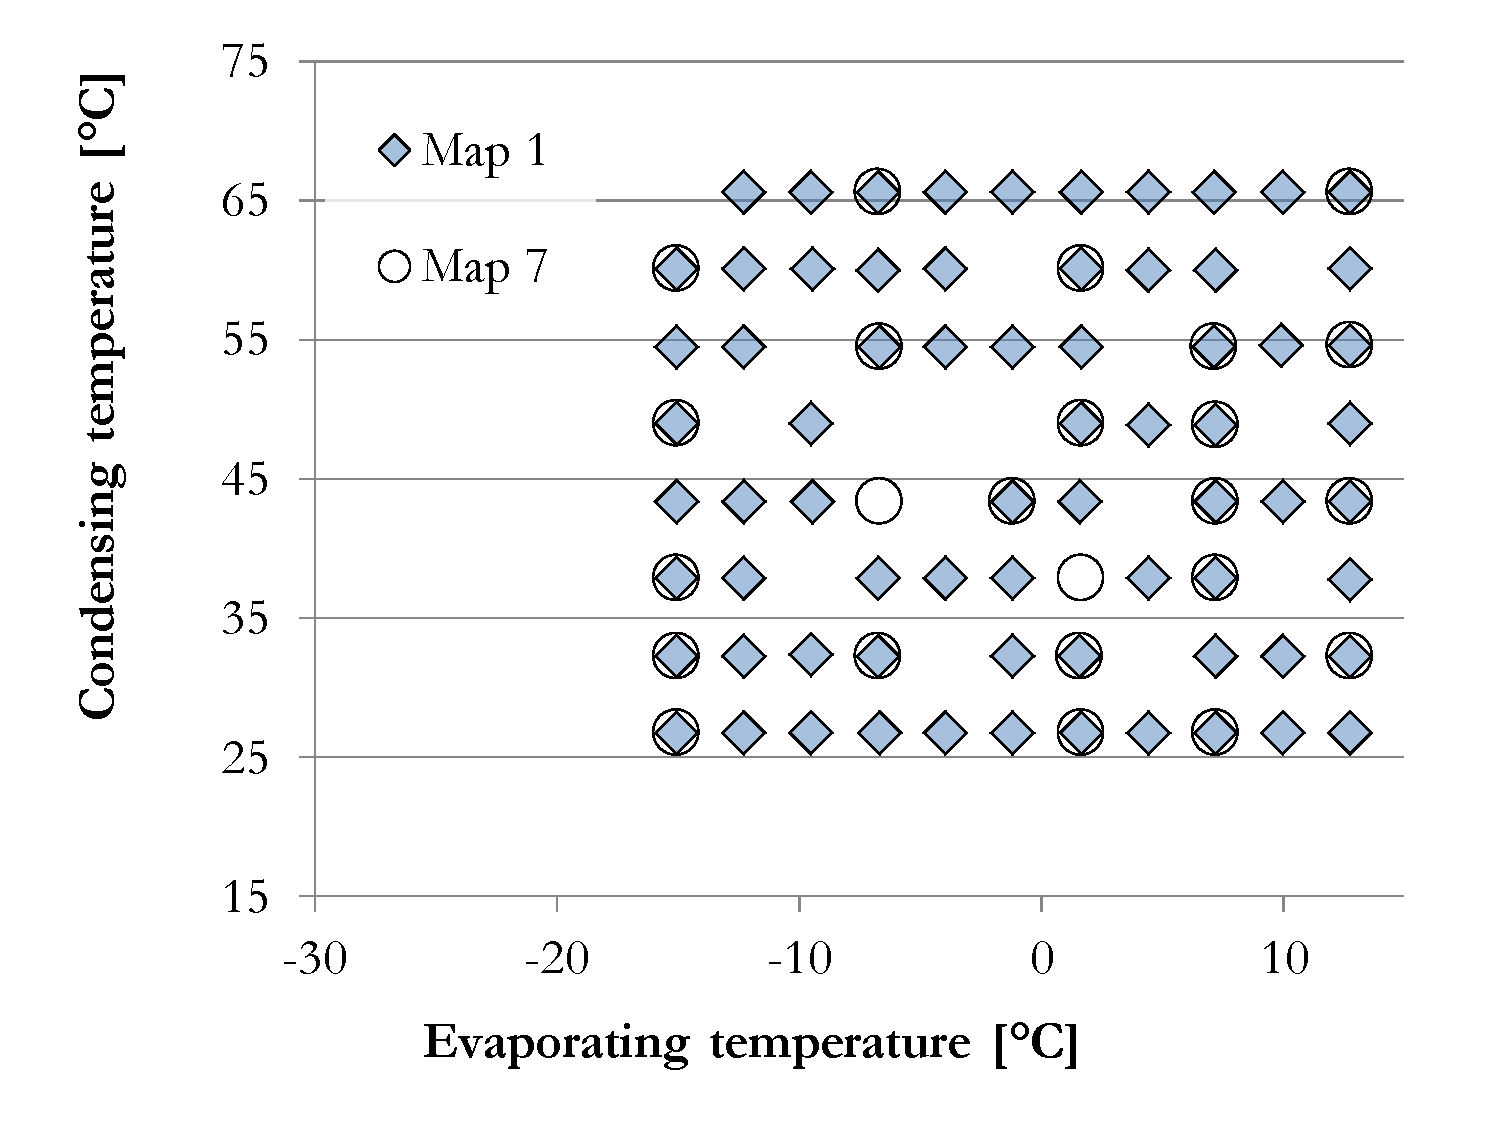
\includegraphics[width=15pc]{./fig/Map_1_and_7_training_data.pdf}
\caption{\label{fig:map_1_7_training_data}Training data points for maps 1 and 7. Note the absence of low temperature training data.}
\end{minipage}\hspace{2pc}%
\begin{minipage}{15pc}
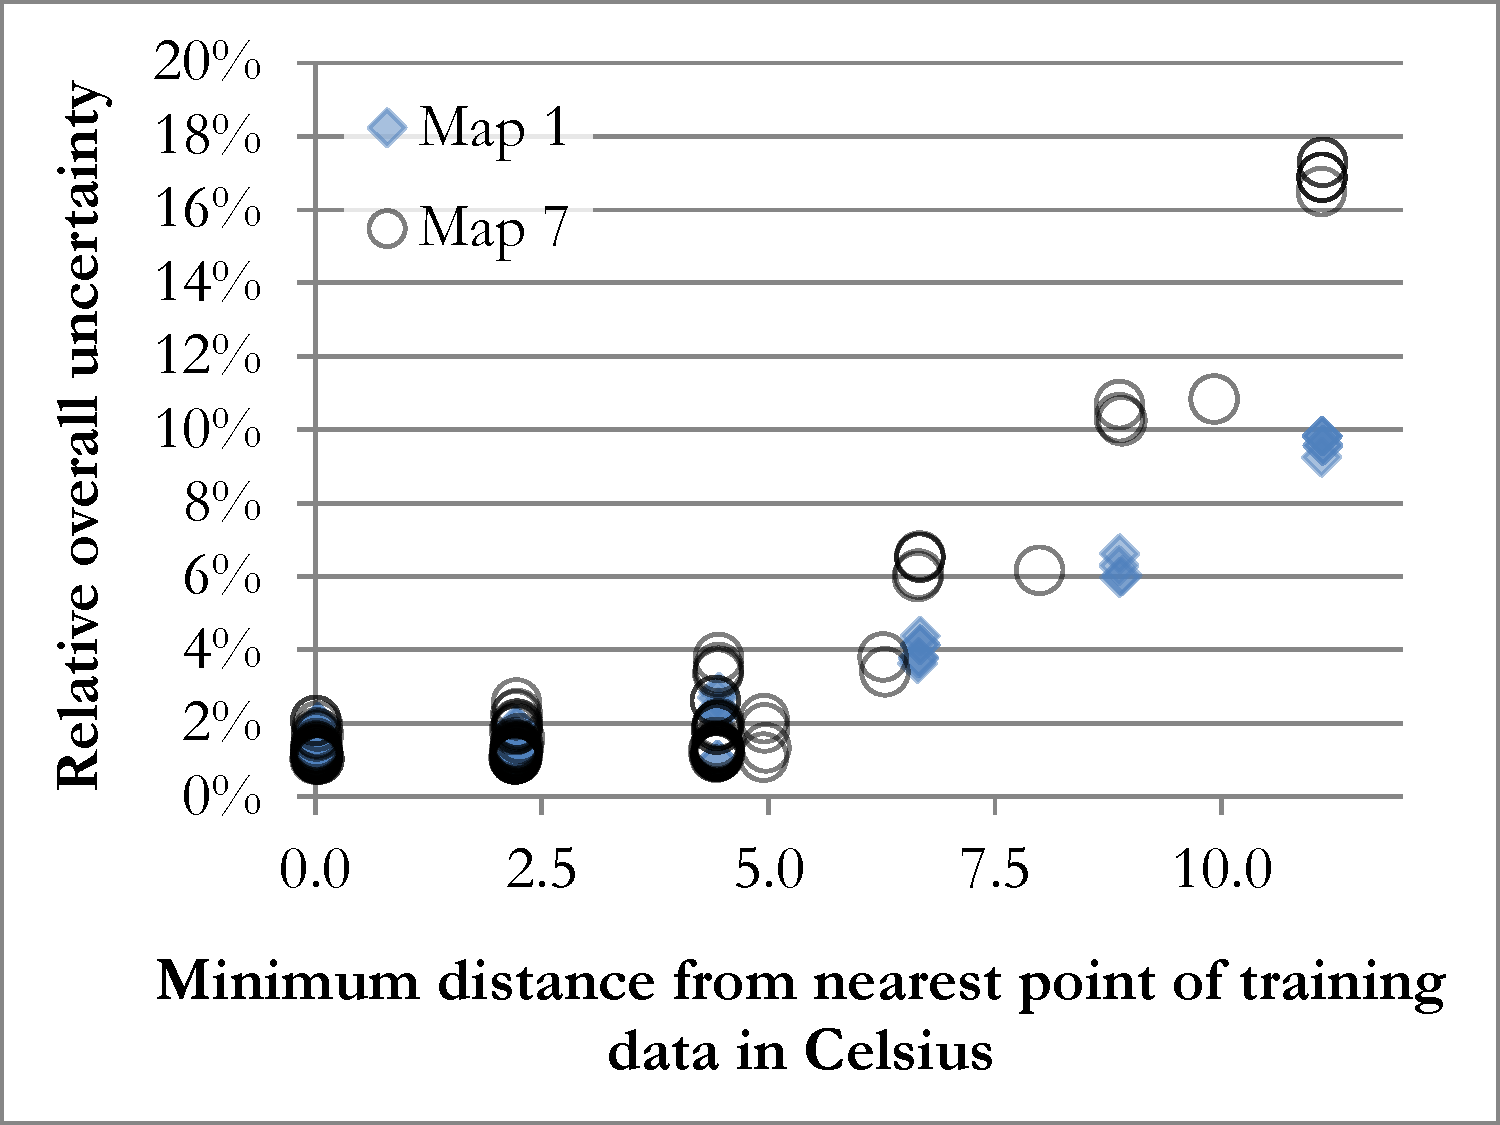
\includegraphics[width=15pc]{./fig/Map_1_and_7_C_distance.pdf}
\caption{\label{fig:map_1_7_unc_C_distance}Change of accuracy with distance to nearest training data point for maps 1 and 7.}
\end{minipage} 
\end{figure}


